%\documentclass[aspectratio=169, handout]{beamer}
\documentclass[aspectratio=169]{beamer}

%%%%%%%%%%%%%%%%%%%%%%%%%%%%%%
% Language and font settings
%%%%%%%%%%%%%%%%%%%%%%%%%%%%%%
\usepackage[english]{babel} % set document language to English

% If the document is not compiled with XeLaTeX, we need to enable input and output for special characters
\usepackage{ifxetex}
\ifxetex
    \usepackage{fontspec} % enables selection of fonts in XeLaTeX
\else
    \usepackage[T1]{fontenc} % to encode glyphs like ä,ö,ü in the output font
    \usepackage{lmodern} % use latin modern font (its prettier!)
\fi

%%%%%%%%%%%%%%%%%%%%%%%%%%%%%%
% Setup various aspects of the layout
%%%%%%%%%%%%%%%%%%%%%%%%%%%%%%
\setlength{\parindent}{0em} % no indentation at the start of paragraphs
\setlength{\parskip}{0.9ex} % create a little distance between paragraphs
\setlength{\fboxsep}{0.6em} % create a bit more distance between an fbox and the text in it

%%%%%%%%%%%%%%%%%%%%%%%%%%%%%%
% Some automatic enhancements for the documents
%%%%%%%%%%%%%%%%%%%%%%%%%%%%%%
\usepackage{microtype} % enables microtype refinements, makes the text body look prettier overall
\usepackage[defaultlines=2, all]{nowidow} % avoids widows (single lines at the top of a page) and orphans (single lines at the bottom of a page)

%%%%%%%%%%%%%%%%%%%%%%%%%%%%%%
% Add commands to fine tune some aspects of the document
%%%%%%%%%%%%%%%%%%%%%%%%%%%%%%
\usepackage{ragged2e} % gives commands \Centering, \RaggedRight, \RaggedLeft (and corresponding environments), which support hyphenation and thus look prettier

%%%%%%%%%%%%%%%%%%%%%%%%%%%%%%
% Setup maths and physics things
%%%%%%%%%%%%%%%%%%%%%%%%%%%%%%
\usepackage{amssymb} % provides a number of symbols
\usepackage{amsmath} % provides enhancements for documents with mathematical formulas, e.g. the align environment
\usepackage{amsfonts} % provides a font with all kinds of mathematical symbols
\usepackage{amsthm} % provides a possibility to define theorem environments

\usepackage{mathtools} % provide several tools for math typesetting as an extension to amsmath
\usepackage{nicefrac} % provides a tool for typesetting inline fractions as a/b
\usepackage{bm} % provides the \bm command to typeset any symbol in bold

\usepackage{tensor} % provides typesetting for tensors
\usepackage{braket} % provides typesetting for braket notation
\usepackage{siunitx} % support to typeset units
\sisetup{
    range-phrase=-,
    range-units=single
} % options for typesetting things like 1-5cm

%%%%%%%%%%%%%%%%%%%%%%%%%%%%%%
% Setup inclusion of graphics
%%%%%%%%%%%%%%%%%%%%%%%%%%%%%%
\usepackage{tikz} % general graphics package for LaTeX

\usepackage{pgfplots} % package to draw axes and labeled plots
\pgfplotsset{compat=1.18} % recommended by pgfplots: set compatibility to the newest version

\usepackage{graphicx} % gives \includegraphics command
\usepackage{epsfig} % use eps files in figures
\graphicspath{{logos/}, {images/}} % setup path for inclusion of images

\usepackage[export]{adjustbox} % give options to \includegraphics to align images (for the two logos in the titlepage)

%%%%%%%%%%%%%%%%%%%%%%%%%%%%%%
% Bibliography
%%%%%%%%%%%%%%%%%%%%%%%%%%%%%%
\usepackage[
    style=numeric-comp,
    sorting=none,
    giveninits=true
]{biblatex} % use biblatex with a numeric (compact) style, given in the order of citation and abbreviation of given names
\addbibresource{bibliography.bib} % include the bibliography (compatible to subfiles!)
\renewbibmacro*{doi+eprint+url}{
    \printfield{doi}
    \newunit\newblock
    \iffieldundef{doi}{
        \usebibmacro{eprint}
        \iffieldundef{eprint}{\usebibmacro{url+urldate}}{}%
    }{}
}% only print URL if there is no DOI

%%%%%%%%%%%%%%%%%%%%%%%%%%%%%%
% Color definitions
%%%%%%%%%%%%%%%%%%%%%%%%%%%%%%
\usepackage{xcolor} % to define and use colors

% Define some custom colors
\definecolor{myred}{HTML}{A3061E}
\definecolor{myblue}{HTML}{003F77}
\definecolor{myyellow}{HTML}{FFBC42}
\definecolor{mygreen}{HTML}{0B6E4F}
\colorlet{myorange}{myyellow!60!myred}
\colorlet{myviolett}{myred!50!myblue!80}

% Define colors from the UHH branding
\definecolor{UHHred}{HTML}{E2001A}
\definecolor{UHHblue}{HTML}{0271BB}
\definecolor{UHHblack}{HTML}{000000}
\definecolor{UHHgray}{HTML}{3B515B}

%%%%%%%%%%%%%%%%%%%%%%%%%%%%%%
% Define environments for code listings
%%%%%%%%%%%%%%%%%%%%%%%%%%%%%%
\usepackage{listings} % to use and define code listings
\lstdefinestyle{python}{
    language=Python,
	basicstyle=\ttfamily,
	keywordstyle=\color{myred},
	identifierstyle=\color{myblue},
	stringstyle=\color{mygreen},
	commentstyle=\color{black!50},
	numberstyle=\color{black!50}\tiny,
	numbers=left,
	belowcaptionskip=\baselineskip,
} % code environment for python code

%%%%%%%%%%%%%%%%%%%%%%%%%%%%%%
% Setup of floats and captions
%%%%%%%%%%%%%%%%%%%%%%%%%%%%%%
\usepackage{caption} % allows control of caption for float environments
\captionsetup{
    font=small,
    format=plain,
    labelfont=bf,
    labelsep=colon,
    margin=10pt,
    textfont=sl,
    singlelinecheck=true,
} % setup the caption for floats

\usepackage{booktabs} % package to typeset prettier tables

%%%%%%%%%%%%%%%%%%%%%%%%%%%%%%
% Things for referencing
%%%%%%%%%%%%%%%%%%%%%%%%%%%%%%
\usepackage{hyperref} % enables use of hyperlinks
\hypersetup{
    linkcolor = UHHblue,
    citecolor  = purple,
    urlcolor   = myblue,
    colorlinks = true,
} % define colors for links

\usepackage{csquotes} % provides \enquote command to do quotes automatically
\usepackage{cleveref} % provides \cref (and \Cref) command, to automatically write out references, depending on the type of reference (figure, equation, etc.)
% must be loaded after hyperref!


\addbibresource{Presentation.bib}

% Basics
%% Sets
\newcommand{\R}{\mathbb{R}}
\newcommand{\Q}{\mathbb{Q}}
\newcommand{\N}{\mathbb{N}}
\newcommand{\C}{\mathbb{C}}

\newcommand{\iu}{\mathrm{i}}

\newcommand{\hateq}{\mathrel{\widehat{=}}}

\DeclareSIUnit{\rydberg}{Ry}
\DeclareSIUnit{\angstrom}{Å}

\DeclareMathOperator{\SPAN}{span}
\DeclareMathOperator{\sign}{sign}

\newcommand{\flatfrac}[2]{\nicefrac{#1}{#2}}

% Vectors
\newcommand{\vb}[1]{\bm{\mathrm{#1}}}
\newcommand{\mat}[1]{\textbf{#1}}
\renewcommand{\vec}[1]{\vb*{#1}}
\newcommand{\ope}[1]{\hat{#1}}


\DeclareMathOperator{\Tr}{Tr}

\title{Superconductivity, flat bands and quantum metric}
\author{Tjark Sievers}
\date{27th June 2024}
\institute[I. ITP - Computational Condensed Matter Theory]{I. Institute of Theoretical Physics}

\usetheme{CCMT}

\begin{document}
	

{
\setbeamertemplate{footline}{\empty}
\begin{frame}
	\titlepage
\end{frame}
}
\addtocounter{framenumber}{-1}

\begin{frame}
	%\begin{itemize}
	%	\item Quarter time of my masters thesis
	%\end{itemize}
	
	\begin{columns}[T]
		\begin{column}{0.5\textwidth}
			\begin{center}
				Hamburg - Computational Condensed Matter Theory
				
				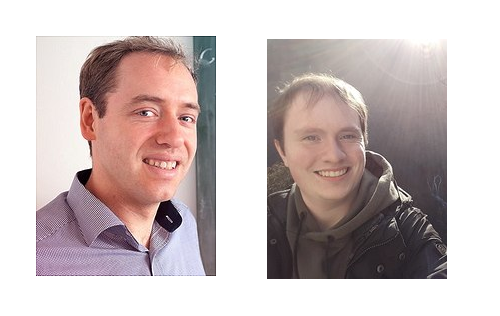
\includegraphics[width=0.8\textwidth]{figs/People Tim.png}
			\end{center}	
		\end{column}
		\begin{column}{0.5\textwidth}
			\begin{center}
				Uppsala - Quantum Matter Theory
				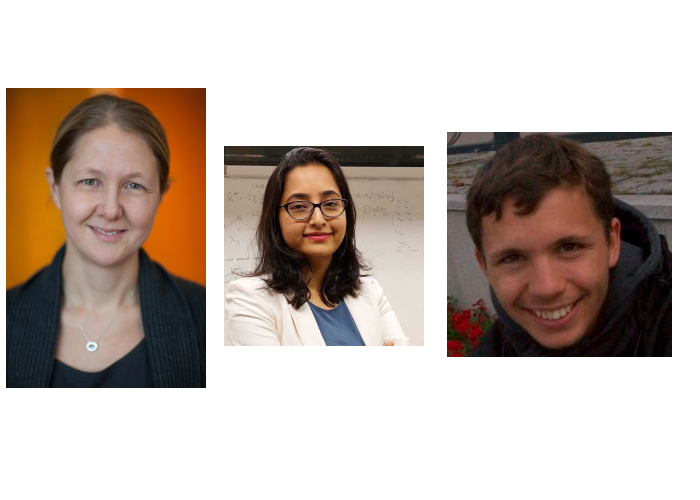
\includegraphics[width=0.9\textwidth]{figs/People Annica.png}
			\end{center}
		\end{column}
	\end{columns}
\end{frame}

\begin{frame}
	\frametitle{Routes to High \(T_{\mathrm{C}}\)}
	
	\begin{columns}[T]
		\begin{column}{0.5\textwidth}
			\begin{center}
				Explore classes of materials that show high \(T_{\mathrm{C}}\) (e.g. Cuprates)
				
				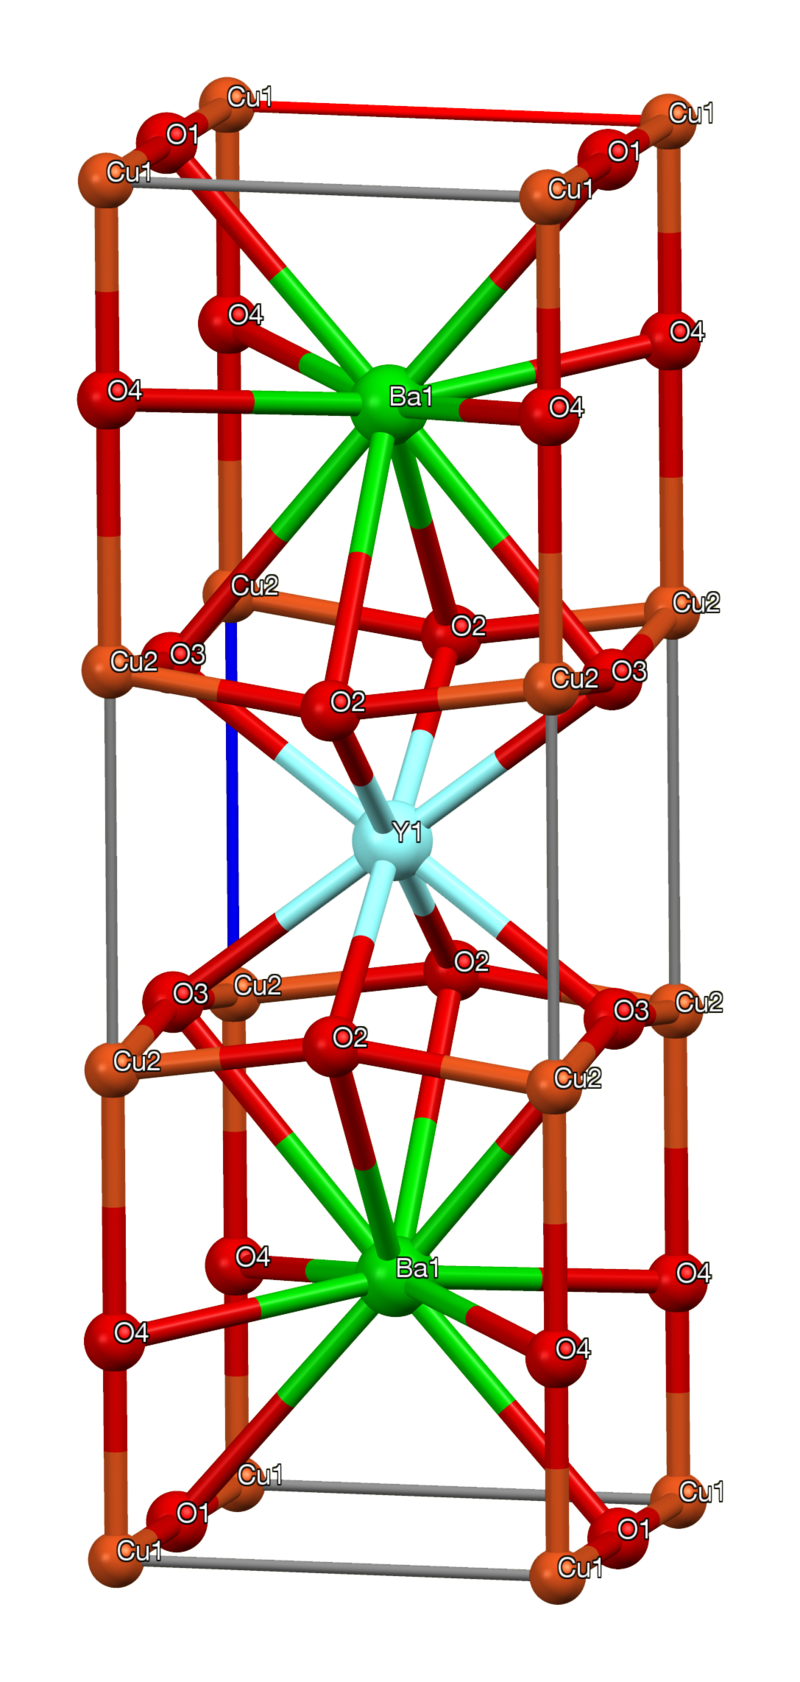
\includegraphics[height=0.4\textheight]{figs/YBCO-xtal-unit-cell-3D-bs-17-atoms-labelled}
				
				YBCO unit cell\footnote<1->[frame]{By Ben Mills - Own work, Public Domain, \href{commons.wikimedia.org/w/index.php?curid=102396546}{Wikimedia Commons}}
			\end{center}
		\end{column}\pause
		\begin{column}{0.5\textwidth}
			\begin{center}
				Simple, tunable systems based on flat bands
				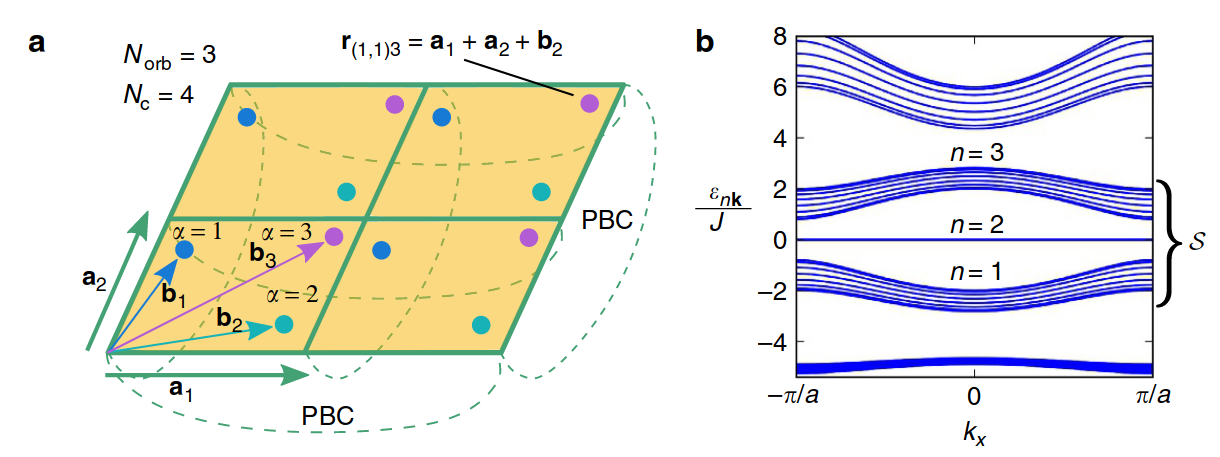
\includegraphics[width=0.95\textwidth]{figs/Lieb lattice}
				Harper-Hubbard model\footnote<2->[frame]{\citeauthor{peottaSuperfluidityTopologicallyNontrivial2015}, \href{https://doi.org/10.1038/ncomms9944}{10.1038/ncomms9944} (\citeyear{peottaSuperfluidityTopologicallyNontrivial2015})}
			\end{center}
		\end{column}
	\end{columns}
\end{frame}

\begin{frame}
	\frametitle{Why Flat Bands?}
	
	BCS theory for dispersive bands:
	\begin{equation}
		T_C \propto \exp{\left(- \frac{1}{U n_0 (E_{\mathrm{F}})}\right)}
	\end{equation}\pause
	
	In flat bands it is predicted:
	\begin{equation}
		T_C \propto U
	\end{equation}
	Exponentially enhanced in comparison to dispersive bands\pause
	
	Due to:
	\begin{itemize}
		\item High DOS near Fermi level
		\item Vanishing kinetic energy, interaction effects dominate
	\end{itemize}
\end{frame}

\begin{frame}
	\frametitle{Twisted Bilayer Graphene\footnote[frame]{\citeauthor{caoUnconventionalSuperconductivityMagicangle2018},  \href{https://doi.org/10.1038/nature26160}{10.1038/nature26160} (\citeyear{caoUnconventionalSuperconductivityMagicangle2018})}\footnote[frame]{Band structure taken from \citeauthor{tormaSuperconductivitySuperfluidityQuantum2022},  \href{https://doi.org/10.1038/s42254-022-00466-y}{10.1038/s42254-022-00466-y} (\citeyear{tormaSuperconductivitySuperfluidityQuantum2022})}}
	
	Example for tunable flat-band system: flat bands can be tuned by changing the twist angle
	
	\begin{columns}[T]
		\begin{column}{0.5\textwidth}
			\begin{center}
				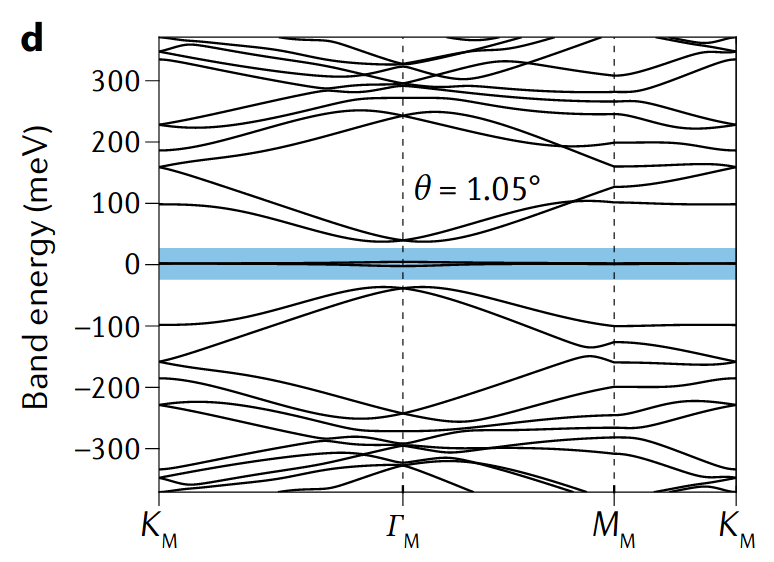
\includegraphics[width=0.8\textwidth]{figs/TBG band structure}
			\end{center}
		\end{column}
		\begin{column}{0.5\textwidth}
			\begin{center}
				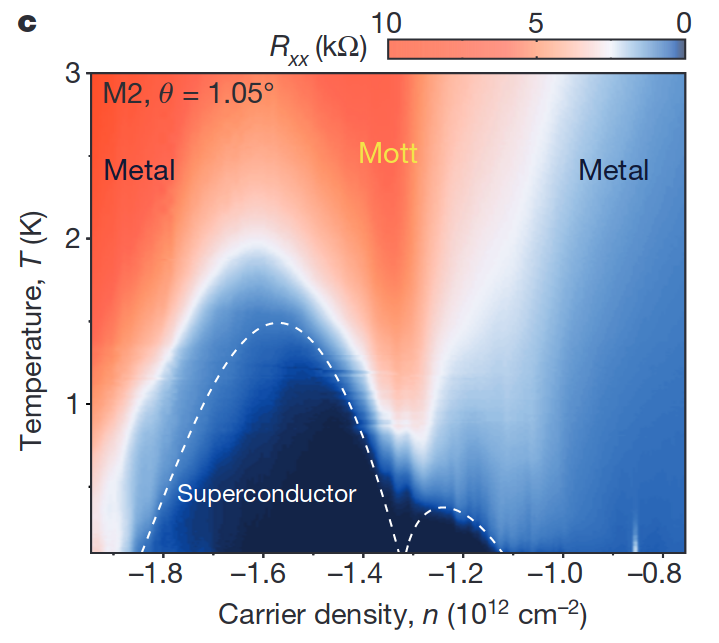
\includegraphics[width=0.8\textwidth]{figs/TBG SC experiment}
			\end{center}
		\end{column}
	\end{columns}
\end{frame}

\begin{frame}
	\frametitle{Transport in Flat-Band Systems}
	
	\begin{block}{}
		\begin{center}
			Below \(T_{\textrm{C}}\), there is pairing.
			Does not necessarily mean there is a supercurrent!
		\end{center}
	\end{block}\pause
	Constitutive equation:
	\begin{equation}
		\vb{j} = -D_{\textrm{S}} \vb{A}
	\end{equation}
	with current density \(\vb{j}\), vector potential \(\vb{A}\), superfluid weight \(D_{\textrm{S}}\).
	Non-zero \(D_{\textrm{S}}\) needed for SC\pause
	
	In single-band BCS theory:
	\begin{equation}
		D_{S, ij} \sim \sum_{\vb{k}} \pdv{\epsilon}{k_i,k_j} \hspace{1cm} \text{Vanishes for a flat band!}
	\end{equation}
\end{frame}


\begin{frame}
	\frametitle{And Yet!}
	
	\begin{center}
		\includegraphics[width=0.6\textwidth]{figs/Peotta Törma 2015 Screenshot}
	\end{center}\pause
	
	Show\footnote<2->[frame]{\footnotesize \citeauthor{peottaSuperfluidityTopologicallyNontrivial2015}, \href{https://doi.org/10.1038/ncomms9944}{10.1038/ncomms9944} (\citeyear{peottaSuperfluidityTopologicallyNontrivial2015})} there are actually 3 terms making up \(D_{\textrm{S}}\):
	
	\begin{itemize}
		\item Conventional:
		\begin{equation}
			D_{\textrm{S}, 1, ij} \sim \sum_{\vb{k}} \pdv{\epsilon}{k_i,k_j}
		\end{equation}\pause
		\item Geometric: 
		\begin{equation}
			D_{\textrm{S}, 2, ij} + D_{\textrm{S}, 3, ij} \sim U \mathcal{M}_{ij}^{\textrm{R}}
		\end{equation}
	\end{itemize}
\end{frame}

\begin{frame}
	\(\mathcal{M}_{ij}^{\textrm{R}}\) related to a quantity called the \textbf{quantum metric} \(g_{ij} (\vb{k})\):
	\begin{equation}
		\mathcal{M}_{ij}^{\textrm{R}} \sim \int_{\textrm{BZ}} \odif[order=2]{\vb{k}} g_{ij} (\vb{k})
	\end{equation}\pause
	In lattice systems:
	\begin{align}
		g_{ij} (\vb{k}) = \Tr{\left[\pdif{i} P(\vb{k}) \pdif{j} P(\vb{k}) \right]} 
	\end{align}
	with projector to the band \(n\) of interest \(P(\vb{k}) = \ket{u_{n \vb{k}}} \bra{u_{n \vb{k}}}\), Bloch functions \(\ket{u_{n \vb{k}}}\)

	%Measures distance between infinitesimally close wavefunctions in \(\vb{k}\)-space\pause
	
	Determining factor for finite quantum metric: mixing between bands\pause
	
	\begin{block}{}
		 \begin{center}
		 	finite quantum metric \pause\(\to\) finite overlap of Wannier functions \\ \pause \(\to\) non-localized Cooper pairs \pause\(\to\) transport in the system is possible
		 \end{center}
	\end{block}
\end{frame}

\begin{frame}
	\frametitle{Wannier Overlap and Transport\footnote[frame]{Graphic from \citeauthor{tormaSuperconductivitySuperfluidityQuantum2022}, \href{https://doi.org/10.1038/s42254-022-00466-y}{10.1038/s42254-022-00466-y} (\citeyear{tormaSuperconductivitySuperfluidityQuantum2022})}}
	
	\begin{center}
		\includegraphics[width=0.7\linewidth]{"figs/Wannier function overlap 1"}
	\end{center}	\pause
	\begin{center}
		\includegraphics[width=0.7\linewidth]{"figs/Wannier function overlap 2"}
	\end{center}
\end{frame}

%\begin{frame}
	%\frametitle{A Connection to Topology}
		
	%Lower bound for \(\mathcal{M}_{ij}^{\textrm{R}}\) given by Chern number \(\mathcal{C}\):
	%\begin{equation}
		%\det{\mathcal{M}_{ij}^{\textrm{R}}} \geq \mathcal{C}^2
	%\end{equation}\pause
	%Explanation for this connection: topological invariants provide obstruction to full localization of Wannier functions
%\end{frame}

\begin{frame}
	\frametitle{Examples}
	
	\begin{columns}[T]
		\begin{column}{0.5\textwidth}
			\begin{center}
				\includegraphics[width=0.8\linewidth]{"figs/Superfluid weight Hexagonal Lattice"}
				
				Hubbard models\footnote[frame]{\citeauthor{liangBandGeometryBerry2017}, \href{https://doi.org/10.1103/PhysRevB.95.024515}{10.1103/PhysRevB.95.024515} (\citeyear{liangBandGeometryBerry2017})} tuned to flat (top) and dispersive band (bottom)
			\end{center}
		\end{column}\pause
		\begin{column}{0.5\textwidth}
			\begin{center}
				\includegraphics[width=0.7\linewidth]{"figs/Superfluid weight TBG"}
				
				Twisted bilayer Graphene\footnote<2->[frame]{\citeauthor{tormaSuperconductivitySuperfluidityQuantum2022}, \href{https://doi.org/10.1038/s42254-022-00466-y}{10.1038/s42254-022-00466-y} (\citeyear{tormaSuperconductivitySuperfluidityQuantum2022})}: geometric contribution overtakes at magic angle \SI{1.05}{\degree}
			\end{center}
		\end{column}
	\end{columns}
\end{frame}

\begin{frame}
	\frametitle{My Model}
	
	\begin{columns}
		\begin{column}{0.4\textwidth}
			\begin{center}
				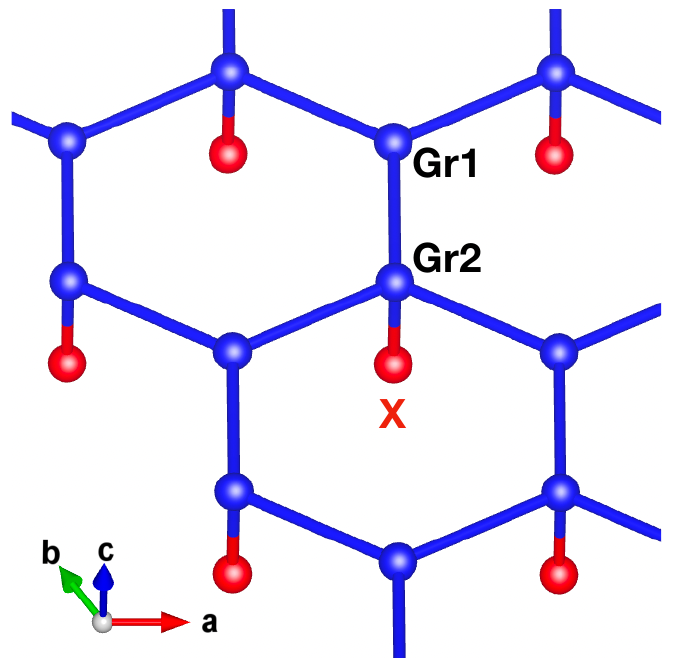
\includegraphics[width=0.6\textwidth]{figs/EG-X structure}
			\end{center}
		\end{column}
		\begin{column}{0.6\textwidth}
			\begin{itemize}
				\item Hexagonal lattice with an additional orbital on one of the sites
				\item Material motivation: Graphene on top of a substrate
			\end{itemize}
		\end{column}
	\end{columns}
	
	Non-interacting Hamiltonian:
	\begin{align}
		H_0 &= -t_{\mathrm{X}} \sum_{\langle ij \rangle, \sigma \sigma^{\prime}} d_{i, \sigma}^{\dagger} d_{j, \sigma^{\prime}}
		-t_{\mathrm{Gr}} \sum_{\langle ij \rangle_{\textrm{Gr}}, \sigma \sigma^{\prime}}
		c_{i, \sigma}^{\dagger} c_{j, \sigma^{\prime}}
		+ V \sum_{i, \sigma \sigma^{\prime}}
		d_{i, \sigma}^{\dagger} c_{i, \sigma^{\prime}}^{(\textrm{Gr2})}
	\end{align}
\end{frame}

\begin{frame}
	Band structure (\(t_{Gr} = 1\), \(t_{X} = 0.01\)):
	
	\begin{figure}
		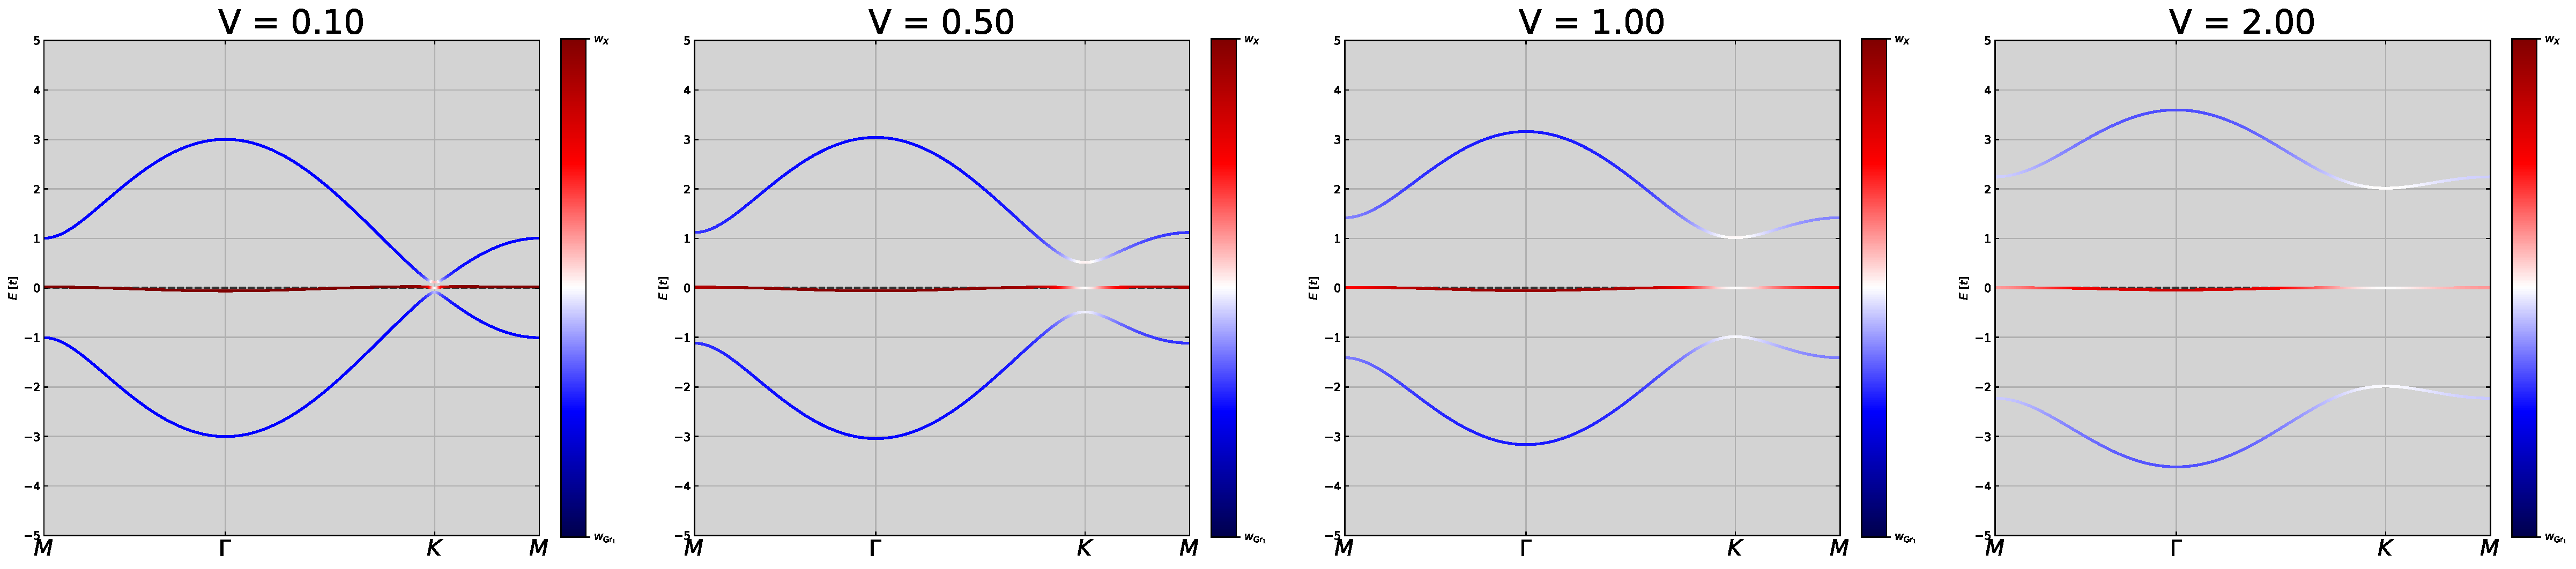
\includegraphics[width=\textwidth]{figs/EG_X bands_tGr_1_tX_0.01}
	\end{figure}\pause
	
	\begin{itemize}
		\item Flat band
		\item Bands are mixed between the Graphene and X orbitals
		\item \(V\) determines this mixing
	\end{itemize}
\end{frame}


\begin{frame}
	Add attractive Hubbard interaction:
	\begin{equation}
		H_{\mathrm{int}} = -U_{\mathrm{X}} \sum_{i} d_{i, \uparrow}^{\dagger} d_{i, \downarrow}^{\dagger} d_{i, \downarrow} d_{i, \uparrow}
		- U_{\mathrm{Gr}} \sum_{i} c_{i, \uparrow}^{\dagger} c_{i, \downarrow}^{\dagger} c_{i, \downarrow} c_{i, \uparrow}
	\end{equation}\pause

	Mean-field decoupling:
	\begin{align}
		H_{\mathrm{int}} \approx \sum_{\alpha, \vb{k}} (\Delta_{\alpha} c_{\vb{k} \alpha \uparrow}^{\dagger} c_{-\vb{k} \alpha \downarrow}^{\dagger} + \Delta_{\alpha}^* c_{-\vb{k} \alpha \downarrow} c_{\vb{k} \alpha \uparrow})
	\end{align}
	with
	\begin{equation}
		\Delta_{\alpha} = - U_{\alpha} \sum_{\vb{k}^{\prime}} \braket{c_{-\vb{k}^{\prime} \alpha \downarrow} c_{\vb{k}^{\prime} \alpha \uparrow}}
	\end{equation}
\end{frame}

\begin{frame}
	Write:
	\begin{equation}
		H_{\mathrm{MF}} = \sum_{\vb{k}} \Psi_{\vb{k}}^{\dagger} \mathcal{H} (\vb{k}) \Psi_{\vb{k}}
	\end{equation}
	with Nambu spinor
	\begin{equation}
		\Psi_{\vb{k}} =
		\begin{pmatrix}
			c_{1, \vb{k} \uparrow} \\
			c_{2, \vb{k} \uparrow} \\
			c_{3, \vb{k} \uparrow} \\
			c_{1, -\vb{k} \downarrow}^{\dagger} \\
			c_{2, -\vb{k} \downarrow}^{\dagger} \\
			c_{3, -\vb{k} \downarrow}^{\dagger} \\
		\end{pmatrix}
	\end{equation}
	and BdG Hamiltonian
	\begin{equation}
		\mathcal{H} (\vb{k}) =
		\begin{pmatrix}
			H_{0, \uparrow} (\vb{k}) - \mu & \Delta \\
			\Delta^{\dagger} & - H_{0, \downarrow}^* (-\vb{k}) + \mu
		\end{pmatrix}
	\end{equation}
\end{frame}

\begin{frame}
	Superfluid weight\footnote{\citeauthor{liangBandGeometryBerry2017}, \href{https://doi.org/10.1103/PhysRevB.95.024515}{10.1103/PhysRevB.95.024515} (\citeyear{liangBandGeometryBerry2017})}:
	\begin{equation}
		D_{\mathrm{S}, ij} = \sum_{\vb{k}} \sum_{m,n,p,q} C_{pq}^{mn} 
		\prescript{}{\uparrow}{\braket{m | \pdif{i} H_{0 \uparrow} (\vb{k}) | n}_{\uparrow}} \prescript{}{\downarrow}{\braket{q | \pdif{j} H_{0 \downarrow} (-\vb{k}) | p}_{\downarrow}}
	\end{equation}
	\(C_{pq}^{mn}\) depends on eigenvalues/eigenvectors of the BdG Hamiltonian, \(\ket{m}_{\sigma}\) are the Bloch functions\pause
	
	Self-consistently find \(\Delta_{\alpha}\): minimize free energy
	\begin{equation}
		F = - \sum_{\vb{k}, i\in \mathrm{occ}} \vert E_{\vb{k}, i} \vert + \sum_{\alpha} \frac{\vert \Delta_{\alpha} \vert^2}{U_{\alpha}}
	\end{equation}
\end{frame}

\begin{frame}[t]
	\frametitle{Results}
	
	\begin{center}
		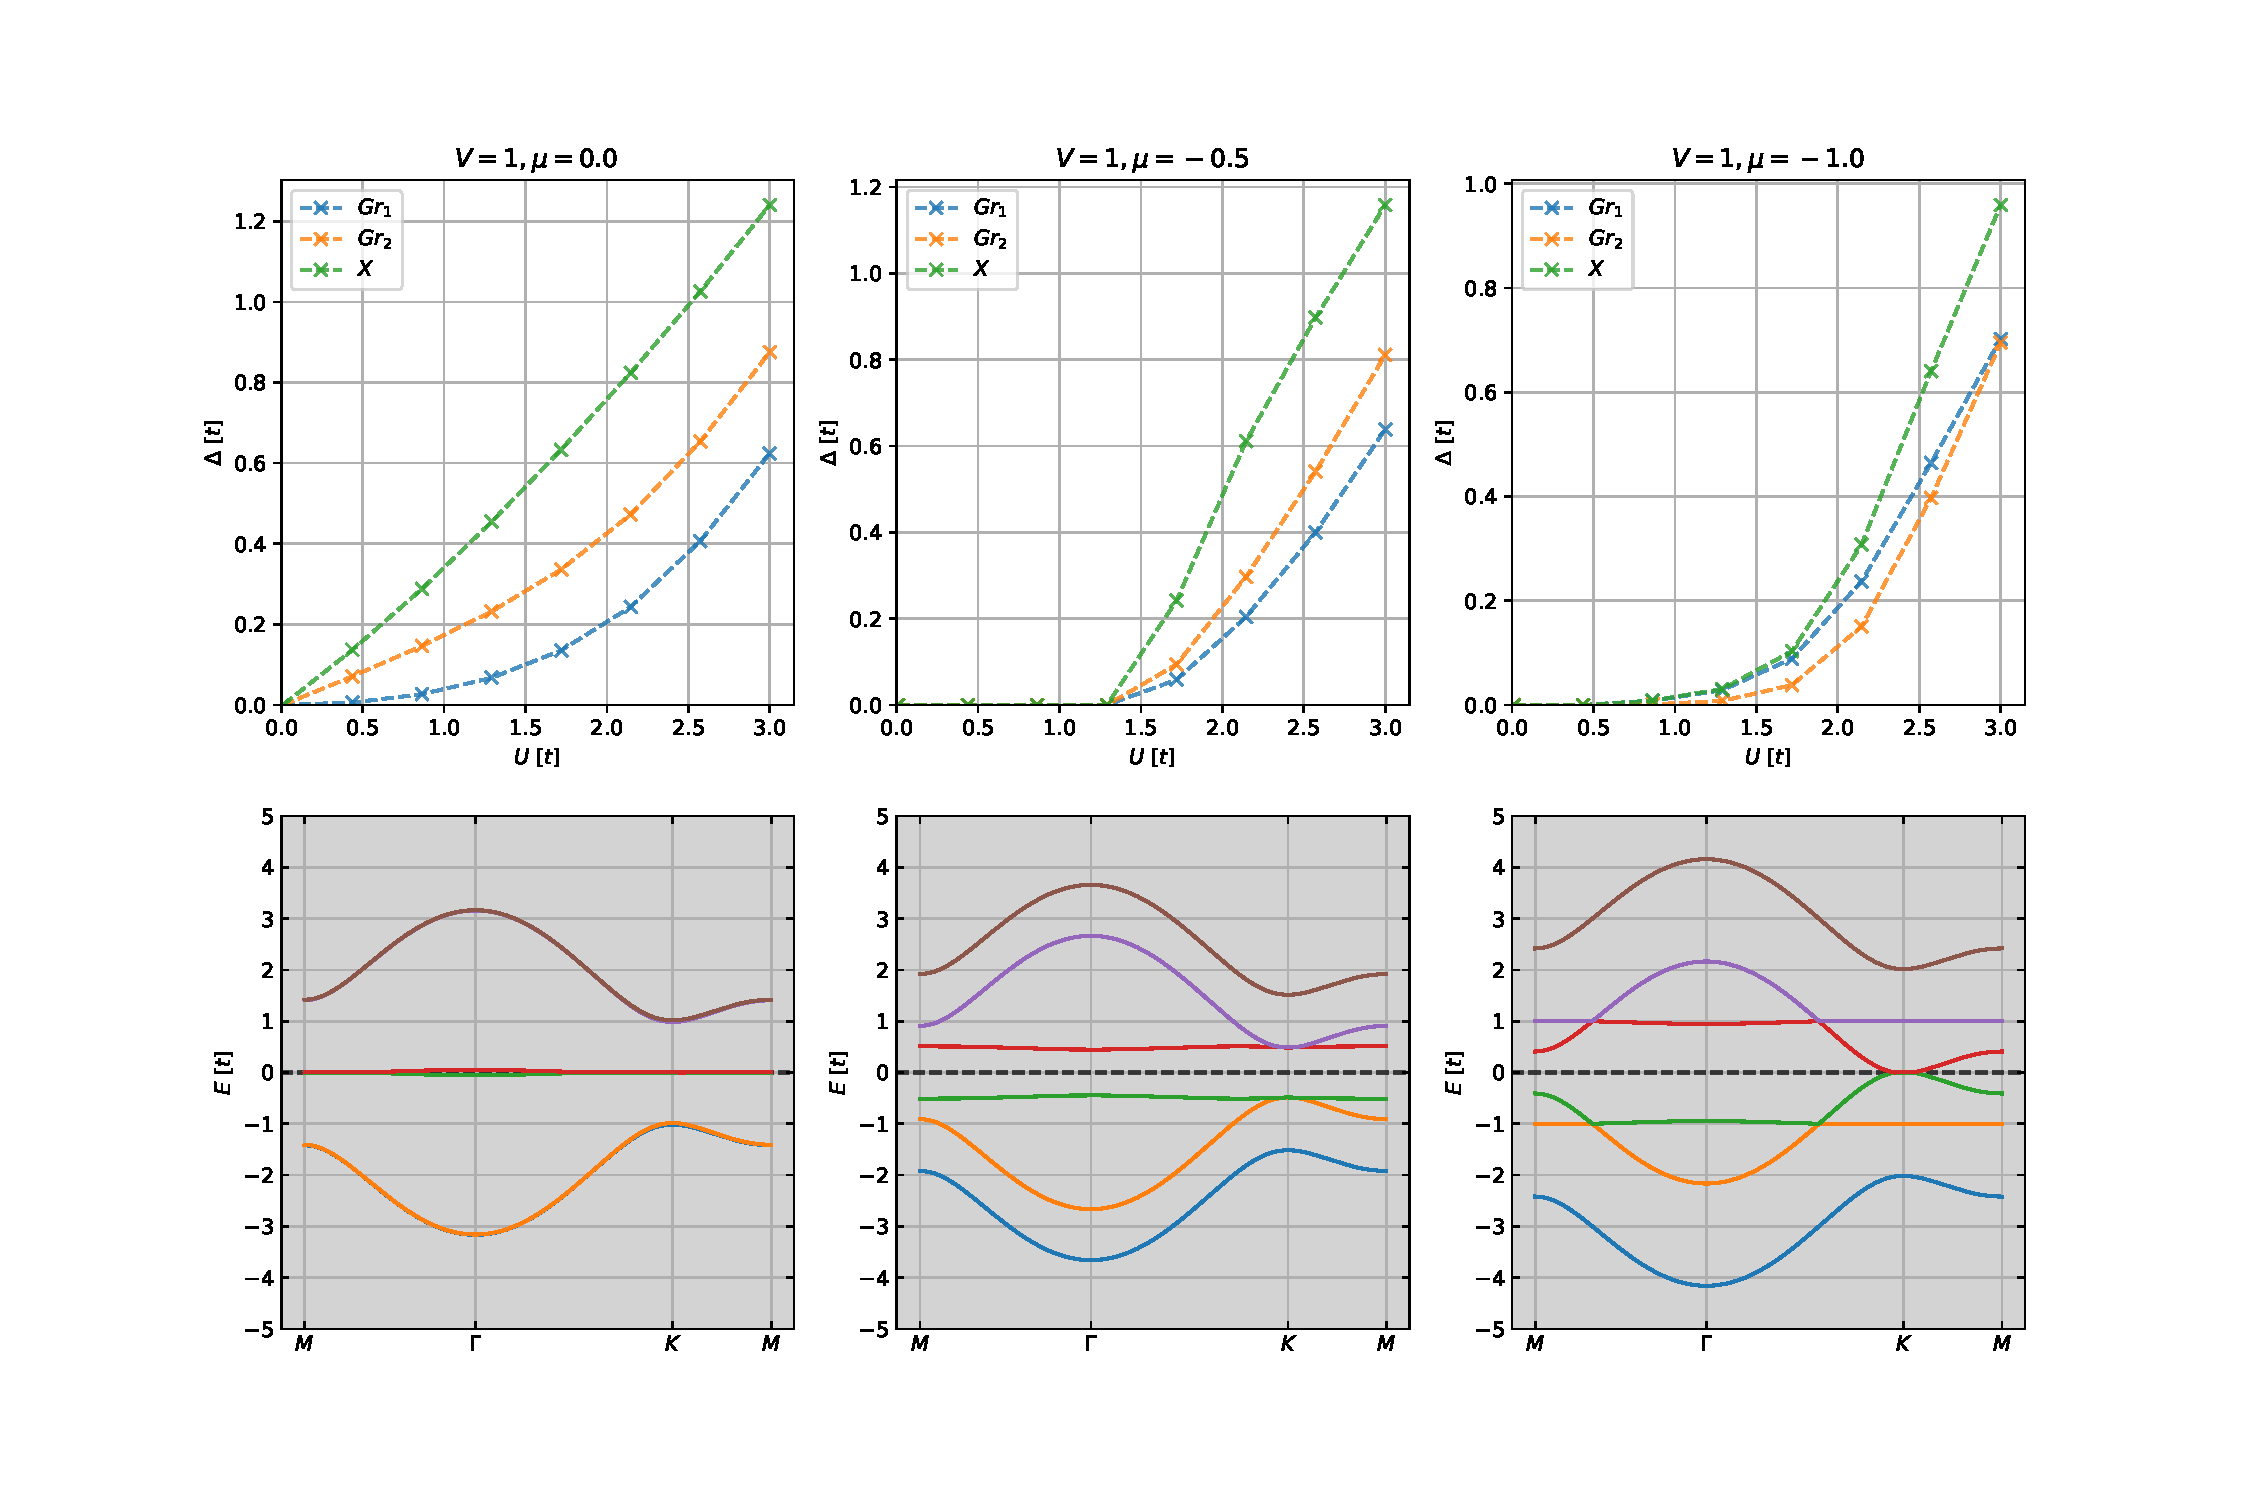
\includegraphics[width=0.65\linewidth]{figs/gap_size_vs_U_egx_uniform_U_V_1}
	\end{center}
\end{frame}

\begin{frame}[t]
	\frametitle{Results}
	
	\begin{center}
		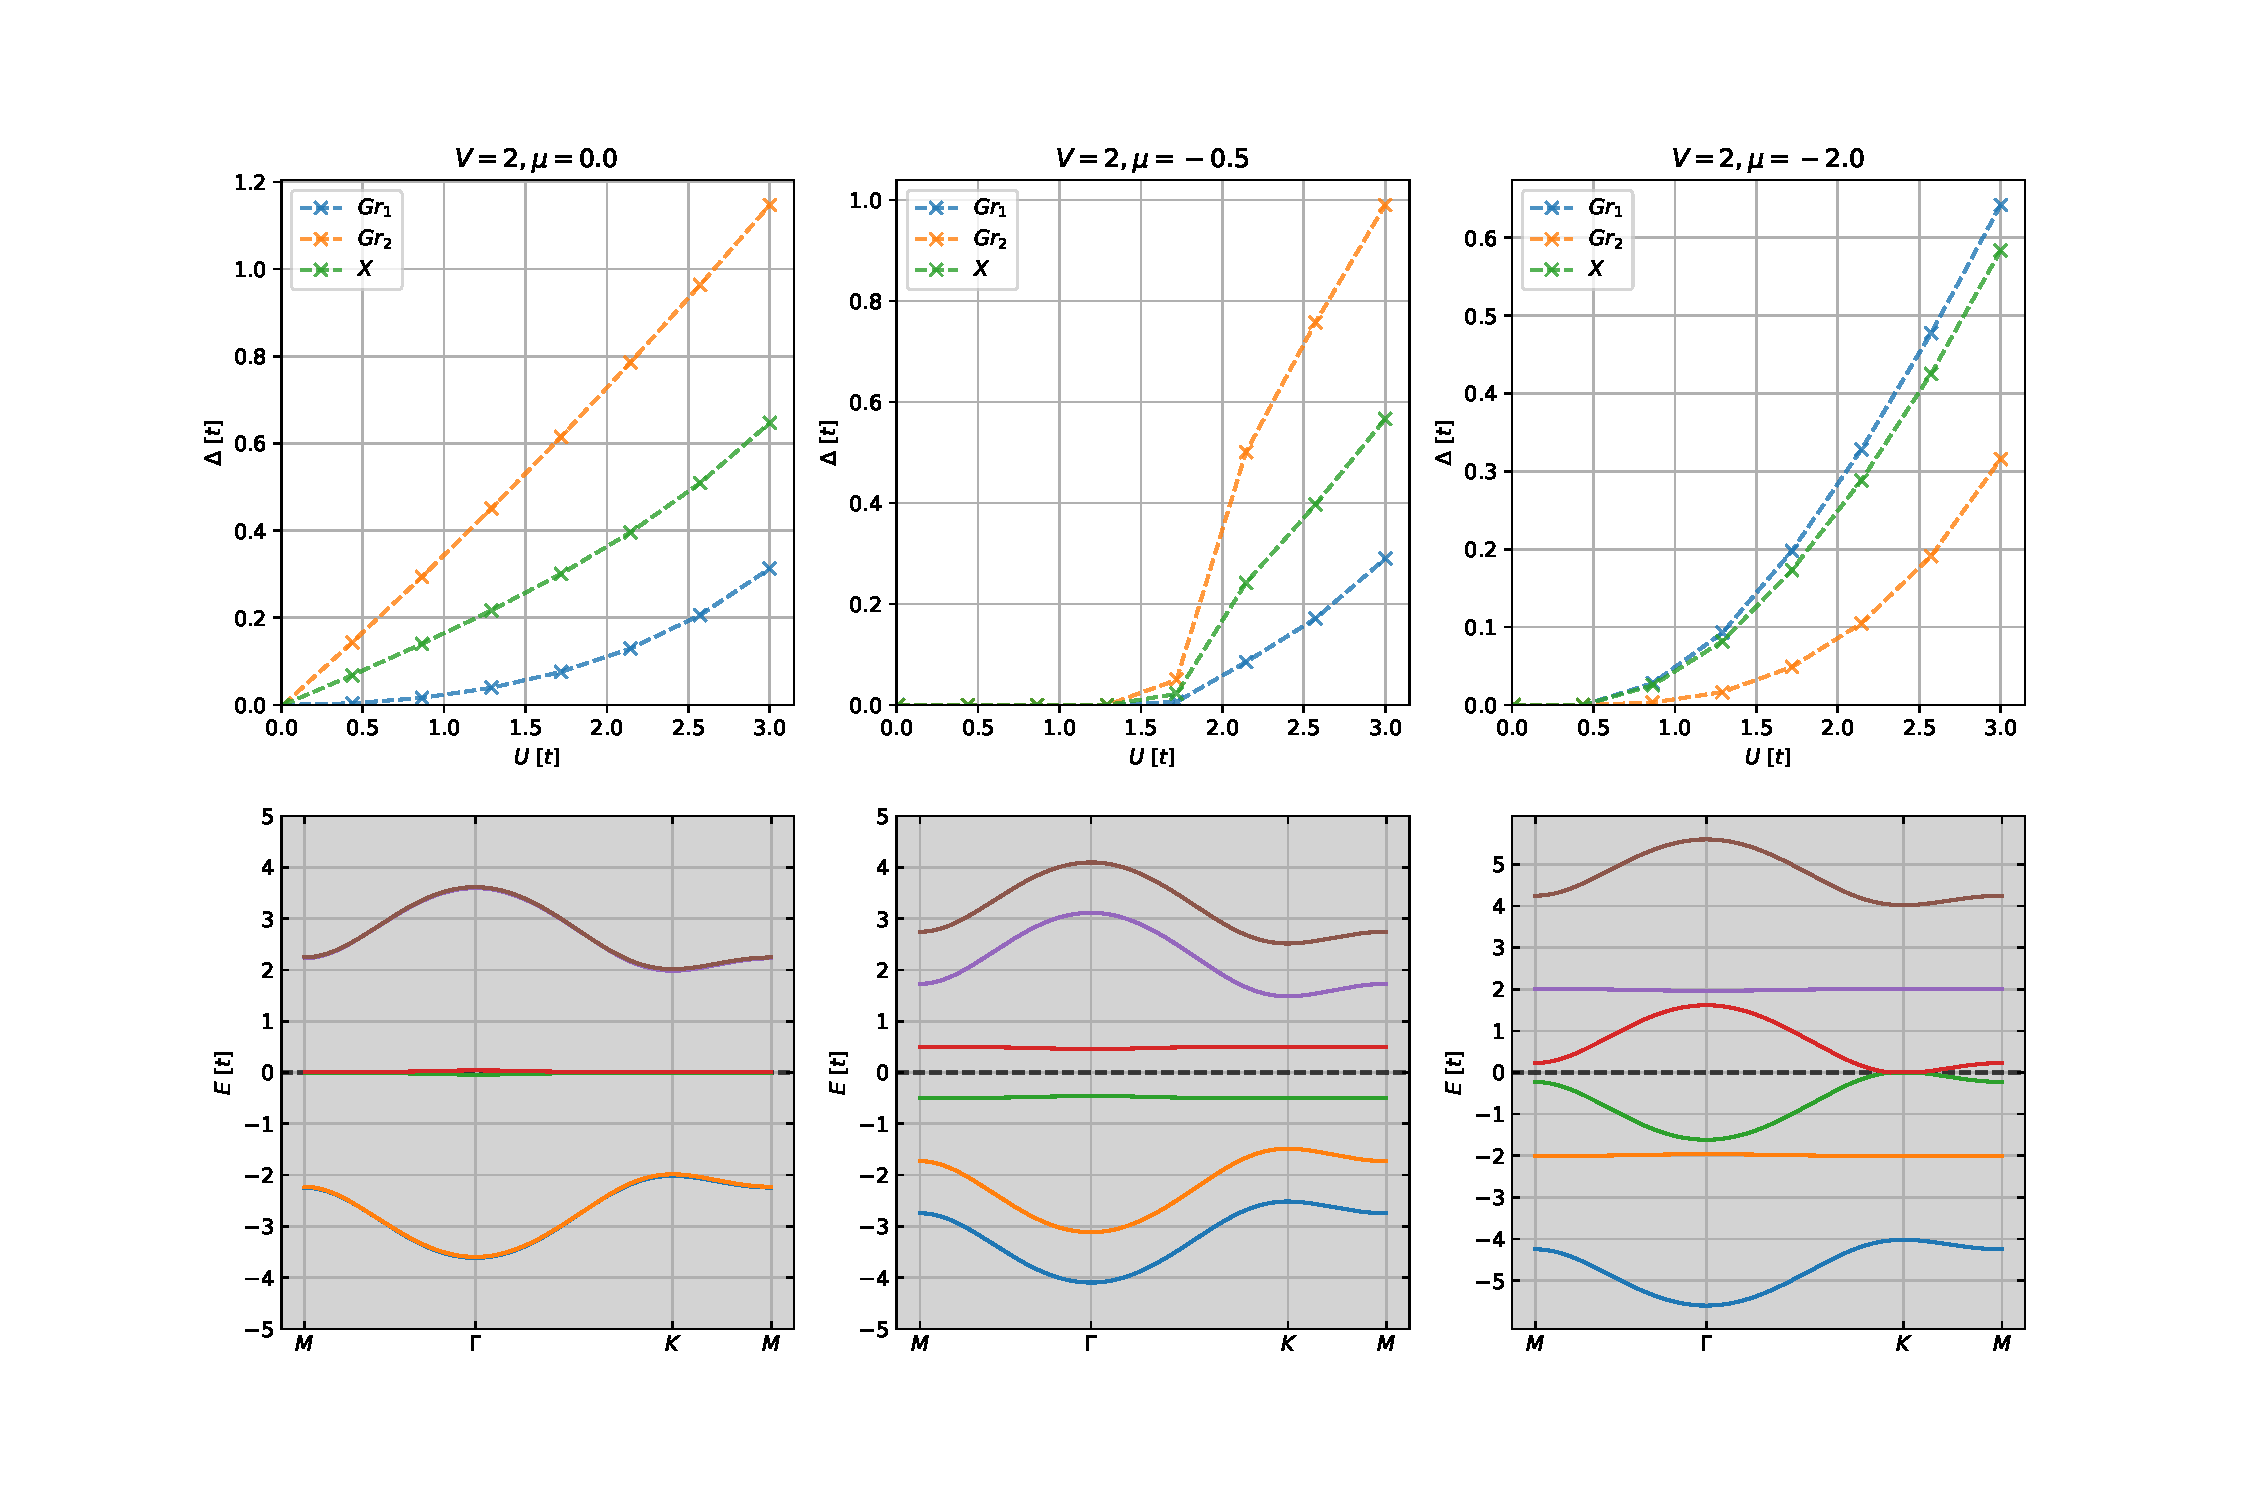
\includegraphics[width=0.65\linewidth]{figs/gap_size_vs_U_egx_uniform_U_V_2}
	\end{center}
\end{frame}


%\begin{frame}
	%\frametitle{Outlook}
	
	%Newer work shows\footnote[frame]{\citeauthor{huhtinenRevisitingFlatBand2022}, \href{https://doi.org/10.1103/PhysRevB.106.014518}{10.1103/PhysRevB.106.014518} (\citeyear{huhtinenRevisitingFlatBand2022})}: connection with 
%\end{frame}

\begin{frame}
	\frametitle{Outlook}
	
	\begin{center}
		\includegraphics[width=0.7\linewidth]{"figs/Pentillä 2022 Paper Screenshot"}
	\end{center}
\end{frame}

\begin{frame}
	\begin{center}
		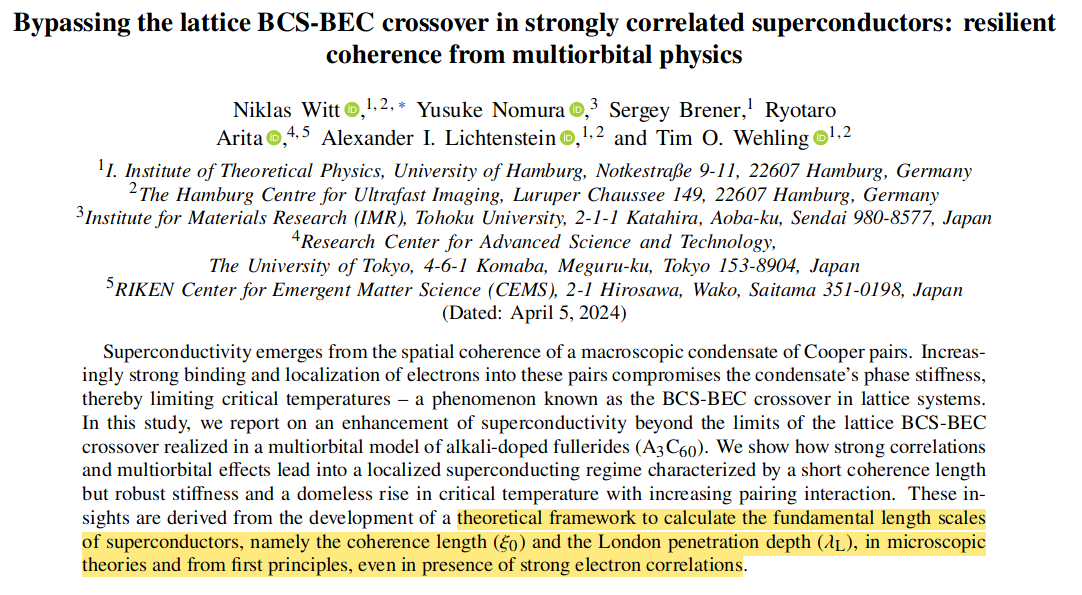
\includegraphics[width=0.7\textwidth]{figs/Witt 2024 Paper Screenshot}
	\end{center}
\end{frame}

\begin{frame}
	
	\begin{center}
		\includegraphics[width=\textwidth]{figs/Pentillä 2024 Paper Screenshot}
	\end{center}
\end{frame}

%\begin{frame}
%	\frametitle{Suggestions for Hamburg after 3 months in Sweden}
%\end{frame}

\begin{frame}
	\frametitle{Summary}
	
	\begin{itemize}
		\item System with flat bands promise high \(T_{\mathrm{C}}\) superconductivity\pause
		\item Superfluid weight (\(\hat{=}\) capacity to host supercurrent) is determined by quantum geometry\pause
		\item Quantum geometry: distances in the space formed by electronic Bloch functions\pause
		\item My work so far: solved system for SC gap self-consistently, found that the pairing is different in the three orbitals
	\end{itemize}	
\end{frame}

%\begin{frame}
	%\frametitle{Quantum metric general}
	
	%Introduction:
	
	%Take Hamiltonian \(\{H(\lambda)\}\) with dependence on some parameters \(\lambda = (\lambda_1, \lambda_2, \ldots)\)
	
	%Have eigenenergies \(E_n (\lambda)\) and eigenstates \(\ket{\phi_n (\lambda)}\)
	
	%Upon infinitesimally varying \(\odif{\lambda}\), define quantum distance:
	%\begin{align}
		%\odif{s}^2 &= \vert \vert \psi (\lambda + \odif{\lambda}) \vert \vert^2 = \braket{\fdif{\psi} | \fdif{\psi}} = \braket{\pdif*{\mu} \psi | \pdif*{\nu} \psi} \odif{\lambda^{\mu}} \odif{\lambda^{\nu}} \\
		%&= (\gamma_{\mu \nu} + \iu \sigma_{\mu \nu}) \odif{\lambda^{\mu}} \odif{\lambda^{\nu}}
	%\end{align}
	%To ensure that gauge invariance, add term:
	%\begin{equation}
		%g_{\mu \nu} (\lambda) \coloneqq \gamma_{\mu \nu} (\lambda) - \beta_{\mu} (\lambda) \beta_{\nu} (\lambda)
	%\end{equation}
	%with Berry connection \(\beta_{\mu} (\lambda) \iu \braket{\phi(\lambda) | \pdif{\mu} \phi(\lambda)}\)
	
	%For two states \(\lambda_I\) and \(\lambda_F\), quantum distance between them:
	%\begin{align}
		%\vert \braket{\psi (\lambda_F) | \psi(\lambda_I)} \vert = 1 - \frac{1}{2} \int_{\lambda_I}^{\lambda_F} g_{\mu \nu} (\lambda) \odif{\lambda^{\mu}} \odif{\lambda^{\nu}}
	%\end{align}
%\end{frame}

\end{document}

